\documentclass{article}

\usepackage[margin=2.5cm,left=2cm,includefoot]{geometry}
\usepackage{graphicx}
\usepackage{float}
\usepackage[space]{grffile}
\usepackage{hyperref}
\usepackage[export]{adjustbox}
\usepackage{multicol}

% Header and footer
\usepackage{fancyhdr}
\pagestyle{fancy}

\rhead{COS301 - \LaTeX}
\lhead{Team Charlie}
\fancyfoot{}
\fancyfoot[R]{Page \thepage}

\renewcommand{\headrulewidth}{2pt}
\renewcommand{\footrulewidth}{1pt}
%

\begin{document}
	
	\begin{titlepage}
		\begin{center}
			
			\line(1,0){300}\\
			[6mm]
			\huge{
				\bfseries Architectural Requirements Notes
			}\\
			[2mm]
			\line(1,0){200}\\
			[15mm]
			\textsc{\large P.A.P.E.R.S (Publication And Papers Electronic Repository System)}\\
			[7.5mm]
			\textsc{\large University of Pretoria - Team Charlie}\\
			[20mm]
			\large{\textbf{Notes By:}}\\
			[2mm]
			\large{
				\href{https://github.com/ClaudioMDS}{Claudio Da Silva - 14205892}\\
				\href{https://github.com/DillonHeins}{Dillon Heins - 14035538}
			}\\
			[4cm]
			
			\href{https://github.com/DillonHeins/Charlie}{\textsc{\Large GitHub Repository - Team Charlie}\\[2mm]
				For more information, please click here}
			
		\end{center}	
		\begin{flushright}
			\textsc{\large 5 March 2016}
		\end{flushright}
	\end{titlepage}
	
	\cleardoublepage
	\thispagestyle{empty}
	\tableofcontents
	\cleardoublepage
	\setcounter{page}{1}
	\section{Architecture requirements}\label{sec:requirements}
	
	\subsection{Architectural scope}\label{subsec:scope}
	
		\begin{figure}[H]
			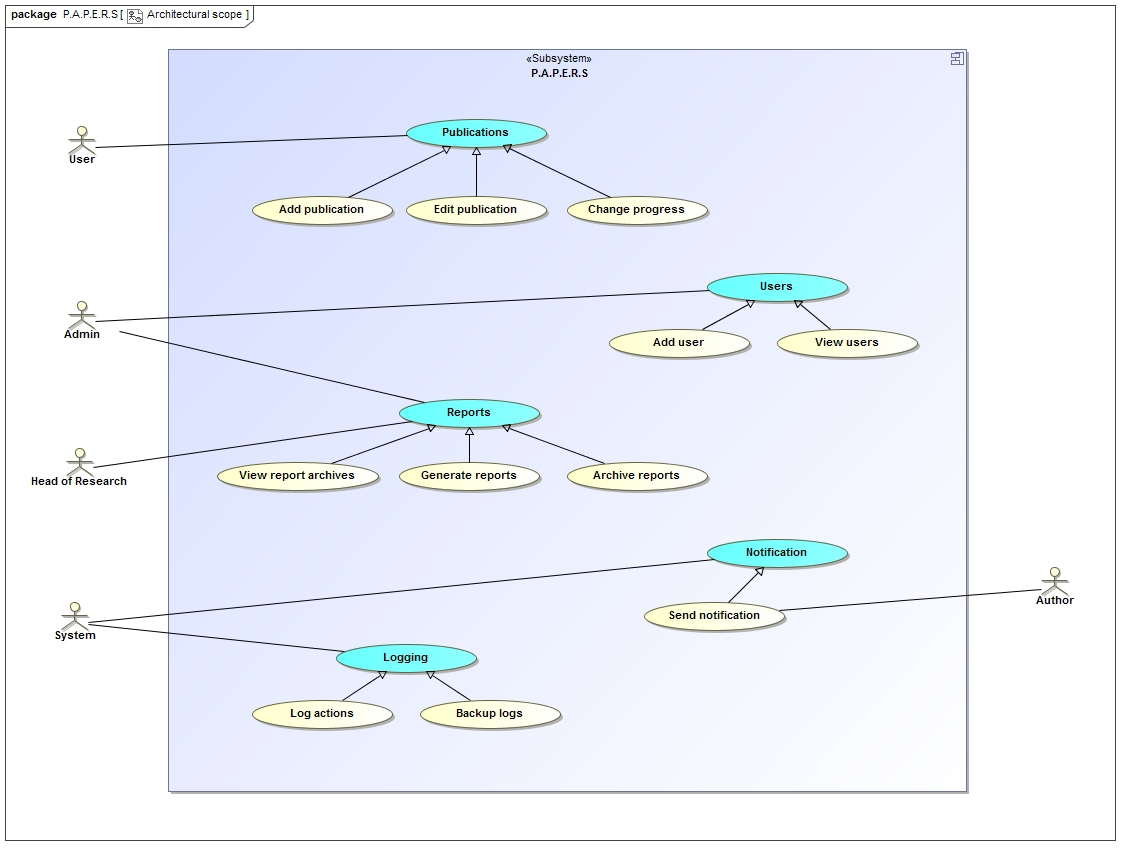
\includegraphics[width=\linewidth]{../../Diagrams/Architectural Scope/Architectural scope.jpg}
			\caption{Architectural Scope - Use case for Architectural Scope (Further refined in use cases)}
		\end{figure}
		
		\par The system will be used to keep track of publications made for various research groups in the department, as well as keep track of the authors and the users in charge of things. From this we may later then generate reports on how various groups are doing as well as the department as a whole, and notify authors and users about upcoming deadlines and events.\\
		
		\par In the event of dealing with queries on database items such as users and publications, for example insertion and deletion, as well as viewing, the system must first validate that those items do or do not exist in said database. Once that is verified, the queries should be run and the result returned. On success the user should be notified, on failure an appropriate exception should be thrown. Persistence must be maintained throughout the database with very little fault tolerance.\\
		
		\par In dealing with reports, data being queried should be validated and the system should ensure that all queried data is recent and correct, halting any new additions during reporting. Reports should be properly archived for later retrieval and properly backed up regularly.\\
		
		\par In dealing with notifications, the system should ensure that all emails being used for every author does in fact exist and is a valid email. When sending this email, likely from the mail server at UP, the SMTP connection used must be ensured to be secured and the email should be sent through valid channels as to not appear as spam mail to other users. The system should also validate that it is using the latest deadline updates at all times.
		
		
		\cleardoublepage
		
	\subsection{Quality requirements}\label{subsec:quality}
		\begin{itemize}
			\item Performance
			\begin{itemize}
				\item Workload is a maximum of 100 users concurrently.
				\item No implementation of concurrent editing of document entries - last saved edit is written to the database.
				\item The system should be able to support 100 users updating information at the same time as updating is more intensive than reading.
				\item The response time of the system should be fast enough that a user is able to complete their work without frustration. Due to the system being off-line it is reasonable to expect the system's response time to be only limited by the speed of the network.
			\end{itemize}
			\item Reliability
			\begin{itemize}
				\item The system should not fail whilst providing critical or important use cases.
				\item The system should handle all requests and respond with appropriate result objects for each.
			\end{itemize}
			\item Scalability
			\begin{itemize}
				\item Ability for multiple external systems to connect to the system's API.
				\item The system should be able to support a large amount of historical document entries being added to the database.
			\end{itemize}
			\item Security
			\begin{itemize}
				\item A hierarchical system will be used to determine the security privileges of users of the system.
				\item Passwords are to be hashed using at least sha256 and should be stored as such within the database along with a salt.
				\item An inactive user session should be terminated after a period of 10 minutes with no activity.
				\item A user who has forgotten their passwords can use a password reset option which will send a one time password to their registered email address so that they may login once using it and reset their password.
			\end{itemize}
			\item Flexibility
			\begin{itemize}
				\item The client has stated that the system is not needed to be able to extend to accommodate a greater number of departments.
			\end{itemize}
			\item Maintainability
			\begin{itemize}
				\item The system should have as few bugs as possible so as to prevent having to constantly maintain it in the future.
				\item The system should be built in a modular way so that all services are decoupled in such a manner that allows for the extension of the system at a later stage.
			\end{itemize}
			\item Auditability/monitorability
			\begin{itemize}
				\item Every action performed by a user should be logged and all details about said action should be stored.
				\item These actions should be visible to admin users.
			\end{itemize}
			\item Integrability
			\begin{itemize}
				\item User's document entries should not be able to be deleted, if it is a case where the document will not be completed it should remain in the system and be terminated.
				\item A user with no admin rights should not have access to admin privileges so that the system's data may remain integrable and safe.
				\item The system should not ever be in a state where it is under pressure and the data is at risk of becoming corrupted. The system should be designed to handle the pressure for which it has been specified to handle.
			\end{itemize}
			\item Cost
			\begin{itemize}
				\item All software used should not be proprietary but rather open source so as to minimise cost as much as possible.
			\end{itemize}
			\item Usability
			\begin{itemize}
				\item The interface should be lightweight.
				\item The interface should be intuitive to use as well as obey Human Computer Interaction guidelines so that it is efficient and easy to use.
			\end{itemize}
		\end{itemize}

		\cleardoublepage
		
	\subsection{Integration and access channel requirements}\label{subsec:integration}
		The system will make use of:
			\begin{itemize}
				\item Django (Model View Controller based framework)
				\item HTML5 compliant front-end to ensure compatibility with Android
				\item Lungo (Android framework based on HTML5 an CSS3)
				\item Sencha Touch (HTML5 Framework for Android)
				\item Android SDK (Final changes to Android app to ensure compatibility)
			\end{itemize}
			
			The different access channels through which the system's services will be made available to users as well as other systems are as follows:
			\begin{itemize}
				\item An Application Program Interface residing on a server which will be interfaced with by clients in order to supply services to them. Clients referring to:
				\begin{itemize}
					\item Human users via an interface
					\item External systems using the services provided by the API
				\end{itemize}
				\item Human users can interface with the system via the use of:
				\begin{itemize}
					\item a web-based application service
					\item an android based mobile application
				\end{itemize}
			\end{itemize}
			The interface is required to be lightweight.

			\cleardoublepage
			
	\subsection{Architectural constraints}\label{subsec:constraints}
		\begin{itemize}
			\item The system should be developed using only non-proprietary technologies.
			\item The system is to be developed for Linux based systems (Mostly Arch Linux) used by the Computer Science department, however preferably the system should run on any general use operating system.
			\item The system should be browser independent, thus the system should be accessed via any browser without issue, including but not limited to (Firefox, Chrome, Safari, Edge etc.)
			\item The system should be handled locally and should not rely on outside internet sources in order to function.
			\item The API created must be queried by both a web browser, as well as an Android application.
			\item The system created should allow for users to use the application via mobile, employing technologies such as bootstrap in order to keep it mobile friendly. This will always allow users of iOS and Windows mobile to access the system via channels such as Safari and Edge.
			\item The system is required to be concurrent and make use of concurrent methods specifically in it's functionality, allowing up to a minimum of a hundred concurrent users to be active at the same time
		\end{itemize}

	
\end{document}
